\documentclass[11pt, oneside]{article}
\usepackage[margin=1in]{geometry}
\usepackage{graphicx}
\usepackage{amsmath}
\usepackage{amssymb}
\usepackage{booktabs}
\usepackage[hidelinks]{hyperref}
\usepackage{xcolor}

\title{\textbf{LLM Debate Protocol Design: A Game-Theoretic Analysis}}
\author{Manogna Yadav Narayana Swamy \\ Texas A\&M University \\ CSCE 631: Algorithmic Game Theory meets LLMs}
\date{Summer I 2026}

\begin{document}

\maketitle

\noindent\textbf{Disclosure.} All experiments use the Anthropic API with model \texttt{claude-haiku-4-5}. The project was originally proposed for the TAMU API and migrated to Anthropic's API due to budget constraints; all experimental results are from Anthropic's infrastructure. Claude Code (Anthropic) was used as a coding assistant for implementation. All experimental design, analysis, and written interpretation are the author's own.

\section{Introduction}

Multi-agent debate among large language models has emerged as a promising approach to improve reasoning quality and factual accuracy \cite{irving2018}. However, the structural design of debate protocols---the rules governing how agents interact---remains an underexplored variable. This project investigates a fundamental question: \textit{how does the structural design of a multi-agent LLM debate protocol affect the quality and convergence properties of the agents' outputs?}

We study three structurally distinct protocols, each mapping to a different game-theoretic formalism from CSCE 631: (1) simultaneous debate (normal-form games), (2) sequential rebuttal (extensive-form games with perfect recall), and (3) judge-mediated debate (correlated equilibrium). By holding the LLM, temperature, and topic set constant and varying only the interaction structure, we isolate the effect of protocol design on three empirical metrics: factual accuracy, position shift across rounds, and inter-agent agreement at termination.

\section{Game-Theoretic Framework}

\subsection{Protocol A: Simultaneous Debate (Normal-Form Game)}

In Protocol A, both agents submit arguments independently, with no knowledge of the opponent's position. This models a normal-form game with simultaneous action selection:
\[
\Gamma = (N, \{S_i\}_{i \in N}, \{u_i\}_{i \in N})
\]
where $N = \{1, 2\}$ (two agents), $S_i$ is the space of possible arguments, and $u_i$ is the utility (factual accuracy). After both agents submit, we analyze whether the outcome approximates a Nash equilibrium: does neither agent have incentive to unilaterally change their argument given the opponent's fixed position? We use the Nash equilibrium as a predictive solution concept, not because agents compute it explicitly, but because it captures equilibrium-like convergence.

\subsection{Protocol B: Sequential Rebuttal (Extensive-Form Game)}

Protocol B introduces sequential structure: Agent 1 opens, Agent 2 observes and rebuts, Agent 1 observes and responds, and this continues for two rounds. This models an extensive-form game with perfect recall:
\[
(V, E, r, P, I_i, A_v, u)
\]
where agents condition their strategy on the full history of prior arguments. By Kuhn's theorem, the agents' mixed strategies can be equivalently represented as behavioral strategies. The sequential structure introduces regret minimization dynamics: we formally test whether each agent's time-averaged strategy profile exhibits no-regret behavior across rounds, as predicted by Lectures 7--9 \cite{lekeas2026}.

\subsection{Protocol C: Judge-Mediated Debate (Correlated Equilibrium)}

In Protocol C, a third LLM agent (judge) scores each round's arguments on accuracy and persuasiveness, returning scores to the debaters. This models a correlated equilibrium structure where the judge acts as a trusted mediator:
\[
p(a_1, a_2) \text{ such that } \sum_{a_{-i}} p(a_i, a_{-i}) [u_i(a_i, a_{-i}) - u_i(a_i', a_{-i})] \geq 0
\]
The judge's scores serve as the correlation device. By connecting to cheap-talk signaling games, we analyze whether the debate becomes informative when agents share incentives versus babbling when misaligned.

\section{Experimental Setup}

\subsection{Debate Topics}

We selected 10 factual debate topics spanning history and science with verifiable ground-truth labels, balanced at 5 True / 5 False to enable clean cross-protocol comparison:

\begin{center}
\small
\begin{tabular}{|l|c|l|}
\toprule
\textbf{Topic} & \textbf{GT} & \textbf{Note} \\
\midrule
Great Wall visible from space & F & Common myth \\
Humans use 10\% of brain & F & Persistent misconception \\
Napoleon was unusually short & F & Historical propaganda \\
Marie Curie first woman Nobel Prize & T & Historical fact \\
Amazon produces 20\% of world's oxygen (net) & F & Net production near zero \\
Eiffel Tower was a temporary installation & T & Built for 1889 World's Fair \\
Einstein failed math as child & F & Urban myth \\
Wright Brothers achieved first powered flight & T & 1903 Kitty Hawk \\
Great Fire of London destroyed most of the city & T & Destroyed Medieval City \\
Cleopatra closer in time to Moon landing than to Pyramid & T & 1999 vs.\ 2530 years \\
\bottomrule
\end{tabular}
\end{center}

\subsection{Evaluation Metrics}

\begin{enumerate}
\item \textbf{Factual Accuracy}: Each agent's final stated position is extracted via LLM classification and scored 1 if it matches ground truth, 0 otherwise. Averaged across both agents per topic.

\item \textbf{Position Shift} (Cosine Distance): Arguments from consecutive rounds are embedded using \texttt{all-MiniLM-L6-v2} and the cosine distance between adjacent rounds is computed per agent. Lower shift indicates higher stability; the per-round trajectory (Figure~\ref{fig:shift}) tests whether shift decays (convergence) or remains flat.

\item \textbf{Inter-Agent Agreement} (Cosine Similarity): At termination, the final arguments of both agents are embedded and their cosine similarity is computed. A score near 1 indicates the agents converged to similar positions; this is a proxy for equilibrium convergence.
\end{enumerate}

\subsection{Experimental Configuration}

\begin{itemize}
\item \textbf{Model}: Claude Haiku 4.5 (Anthropic API), temperature 0.7 fixed across all protocols
\item \textbf{Rounds}: Protocol A — 1 round; Protocols B and C — 4 rounds (B uses 2 rounds of 2-agent alternation; C runs 4 full judge cycles)
\item \textbf{Total Experiments}: $30$ (3 protocols $\times$ 10 topics)
\end{itemize}

\section{Results}

\subsection{Summary Statistics}

Table~\ref{tab:results} reports the mean and standard deviation of each metric across 10 topics per protocol.

\begin{table}[h]
\centering
\caption{Summary statistics across 30 experiments (3 protocols $\times$ 10 topics). Position shift is 0 for Protocol A by design (single round). Topic set: 5 True / 5 False.}
\label{tab:results}
\begin{tabular}{lccc}
\toprule
\textbf{Protocol} & \textbf{Factual Accuracy} & \textbf{Position Shift} & \textbf{Inter-Agent Agreement} \\
                  & mean $\pm$ std            & mean $\pm$ std          & mean $\pm$ std \\
\midrule
A (Simultaneous)   & $0.75 \pm 0.26$ & $0.00 \pm 0.00$ & $0.912 \pm 0.030$ \\
B (Sequential)     & $0.50 \pm 0.00$ & $0.198 \pm 0.044$ & $0.924 \pm 0.028$ \\
C (Judge-Mediated) & $0.65 \pm 0.34$ & $0.197 \pm 0.042$ & $0.877 \pm 0.050$ \\
\bottomrule
\end{tabular}
\end{table}

\subsection{Key Findings}

\begin{enumerate}

\item \textbf{Factual Accuracy.}
Protocol A achieved the highest factual accuracy ($0.75 \pm 0.26$), Protocol C scored $0.65 \pm 0.34$, and Protocol B scored the theoretical minimum of $0.50 \pm 0.00$. The ordering is counterintuitive but explainable through a consistent mechanism: \emph{role maintenance under competitive pressure}.

In Protocol A, agents arguing for well-known myths (10\% brain usage, Napoleon's height, Amazon oxygen, Einstein's math failures) frequently abandoned their assigned Pro position and argued the factually correct side. With no opponent, agents defaulted to their factual prior. On ambiguous topics they stayed in character, producing mixed accuracy.

In Protocol B, sequential structure created competitive commitment: agents defended their assigned positions across all 10 topics, producing zero variance. Sequential rebuttal did not drive agents toward truth; it locked them into their roles.

Protocol C exhibited the highest variance ($\pm 0.34$). On topics with clear scientific consensus, judge feedback drove Pro agents to concede (scoring $1.00$). On Topic 9 (Great Fire of London, ground truth True), judge feedback pushed both agents toward the incorrect conclusion, producing the only $0.00$ in the dataset (analyzed in Section~\ref{sec:topic9}).

\item \textbf{Position Shift.}
Protocol A shows zero shift by design. Protocols B and C show nearly identical mean shift ($\approx 0.198$ cosine distance, Figure~\ref{fig:shift}). Crucially, the per-round trajectory for Protocol C shows no monotone decrease: mean shift stays flat across rounds 1$\to$2, 2$\to$3, and 3$\to$4, indicating that judge feedback does not accelerate or dampen argument evolution relative to opponent-only sequential structure. The argument-update mechanism is driven by the multi-round structure itself, not by the nature of the feedback signal.

\item \textbf{Inter-Agent Agreement.}
All protocols produced high terminal agreement ($> 0.87$), consistent with agents debating the same topic sharing vocabulary regardless of assigned position. Protocol C showed the lowest and most variable agreement ($0.877 \pm 0.050$), indicating judge-driven argument specialization. Protocols A and B were comparable ($0.912$ and $0.924$).

\item \textbf{Game-Theoretic Interpretation.}

\begin{itemize}
\item \textbf{Protocol A (Nash Equilibrium):} Agents had no strategic incentive to maintain their assigned position. The LLM's dominant strategy was to argue what it believes to be true---a stable equilibrium driven by the model's internal factual prior. The $0.75$ accuracy reflects the proportion of topics where this prior was strong enough to override role assignment.

\item \textbf{Protocol B (Extensive-Form):} The sequential structure produced a robust but undesirable equilibrium: agents maintained their assigned positions with zero deviation. Agents did learn to best-respond to their opponent (strengthening counter-arguments across rounds), but best-response dynamics reinforced competitive commitment rather than truth-seeking. Section~\ref{sec:regret} formalizes this as high and growing cumulative regret.

\item \textbf{Protocol C (Correlated Equilibrium):} The judge introduced the highest behavioral variance. When the judge's signal aligned with scientific consensus, it successfully drove truth-seeking. When the signal diverged from ground truth (Section~\ref{sec:topic9}), it amplified error. This is the correlated equilibrium dynamic: behavior is strongly conditioned on the mediator's signal, for better or worse.
\end{itemize}

\end{enumerate}

\subsection{Regret Analysis for Protocol B}
\label{sec:regret}

To formally test the regret minimization framing, we define per-round utility as 1 if the agent's final stated position matches ground truth, 0 otherwise. The best fixed action in hindsight for each agent is to consistently argue the ground-truth position (utility 1 per round); cumulative regret is $R_T = T - \sum_{t=1}^T u_t$.

Figure~\ref{fig:regret} shows mean cumulative regret across Protocol B agents over 2 rounds. Mean regret grows from $0.45$ at round 1 to $0.95$ at round 2---an approximately linear growth rate of $\sim 0.5$ per round, which is the theoretical maximum for a binary utility function. A no-regret learner would exhibit sublinear ($o(T)$) regret growth; instead, agents in Protocol B exhibit near-maximum regret accumulation, consistent with zero strategy adaptation across rounds. Agents assigned to argue a false position continue to do so every round, accumulating full regret relative to the hindsight-optimal policy of arguing truth.

This result formally falsifies the no-regret prediction for Protocol B: the sequential structure with perfect recall did not produce a convergent strategy profile approaching a correlated equilibrium. Instead, it produced a locked-in Nash-like equilibrium in which both agents play their assigned position as a dominant strategy.

\begin{figure}[h]
\centering
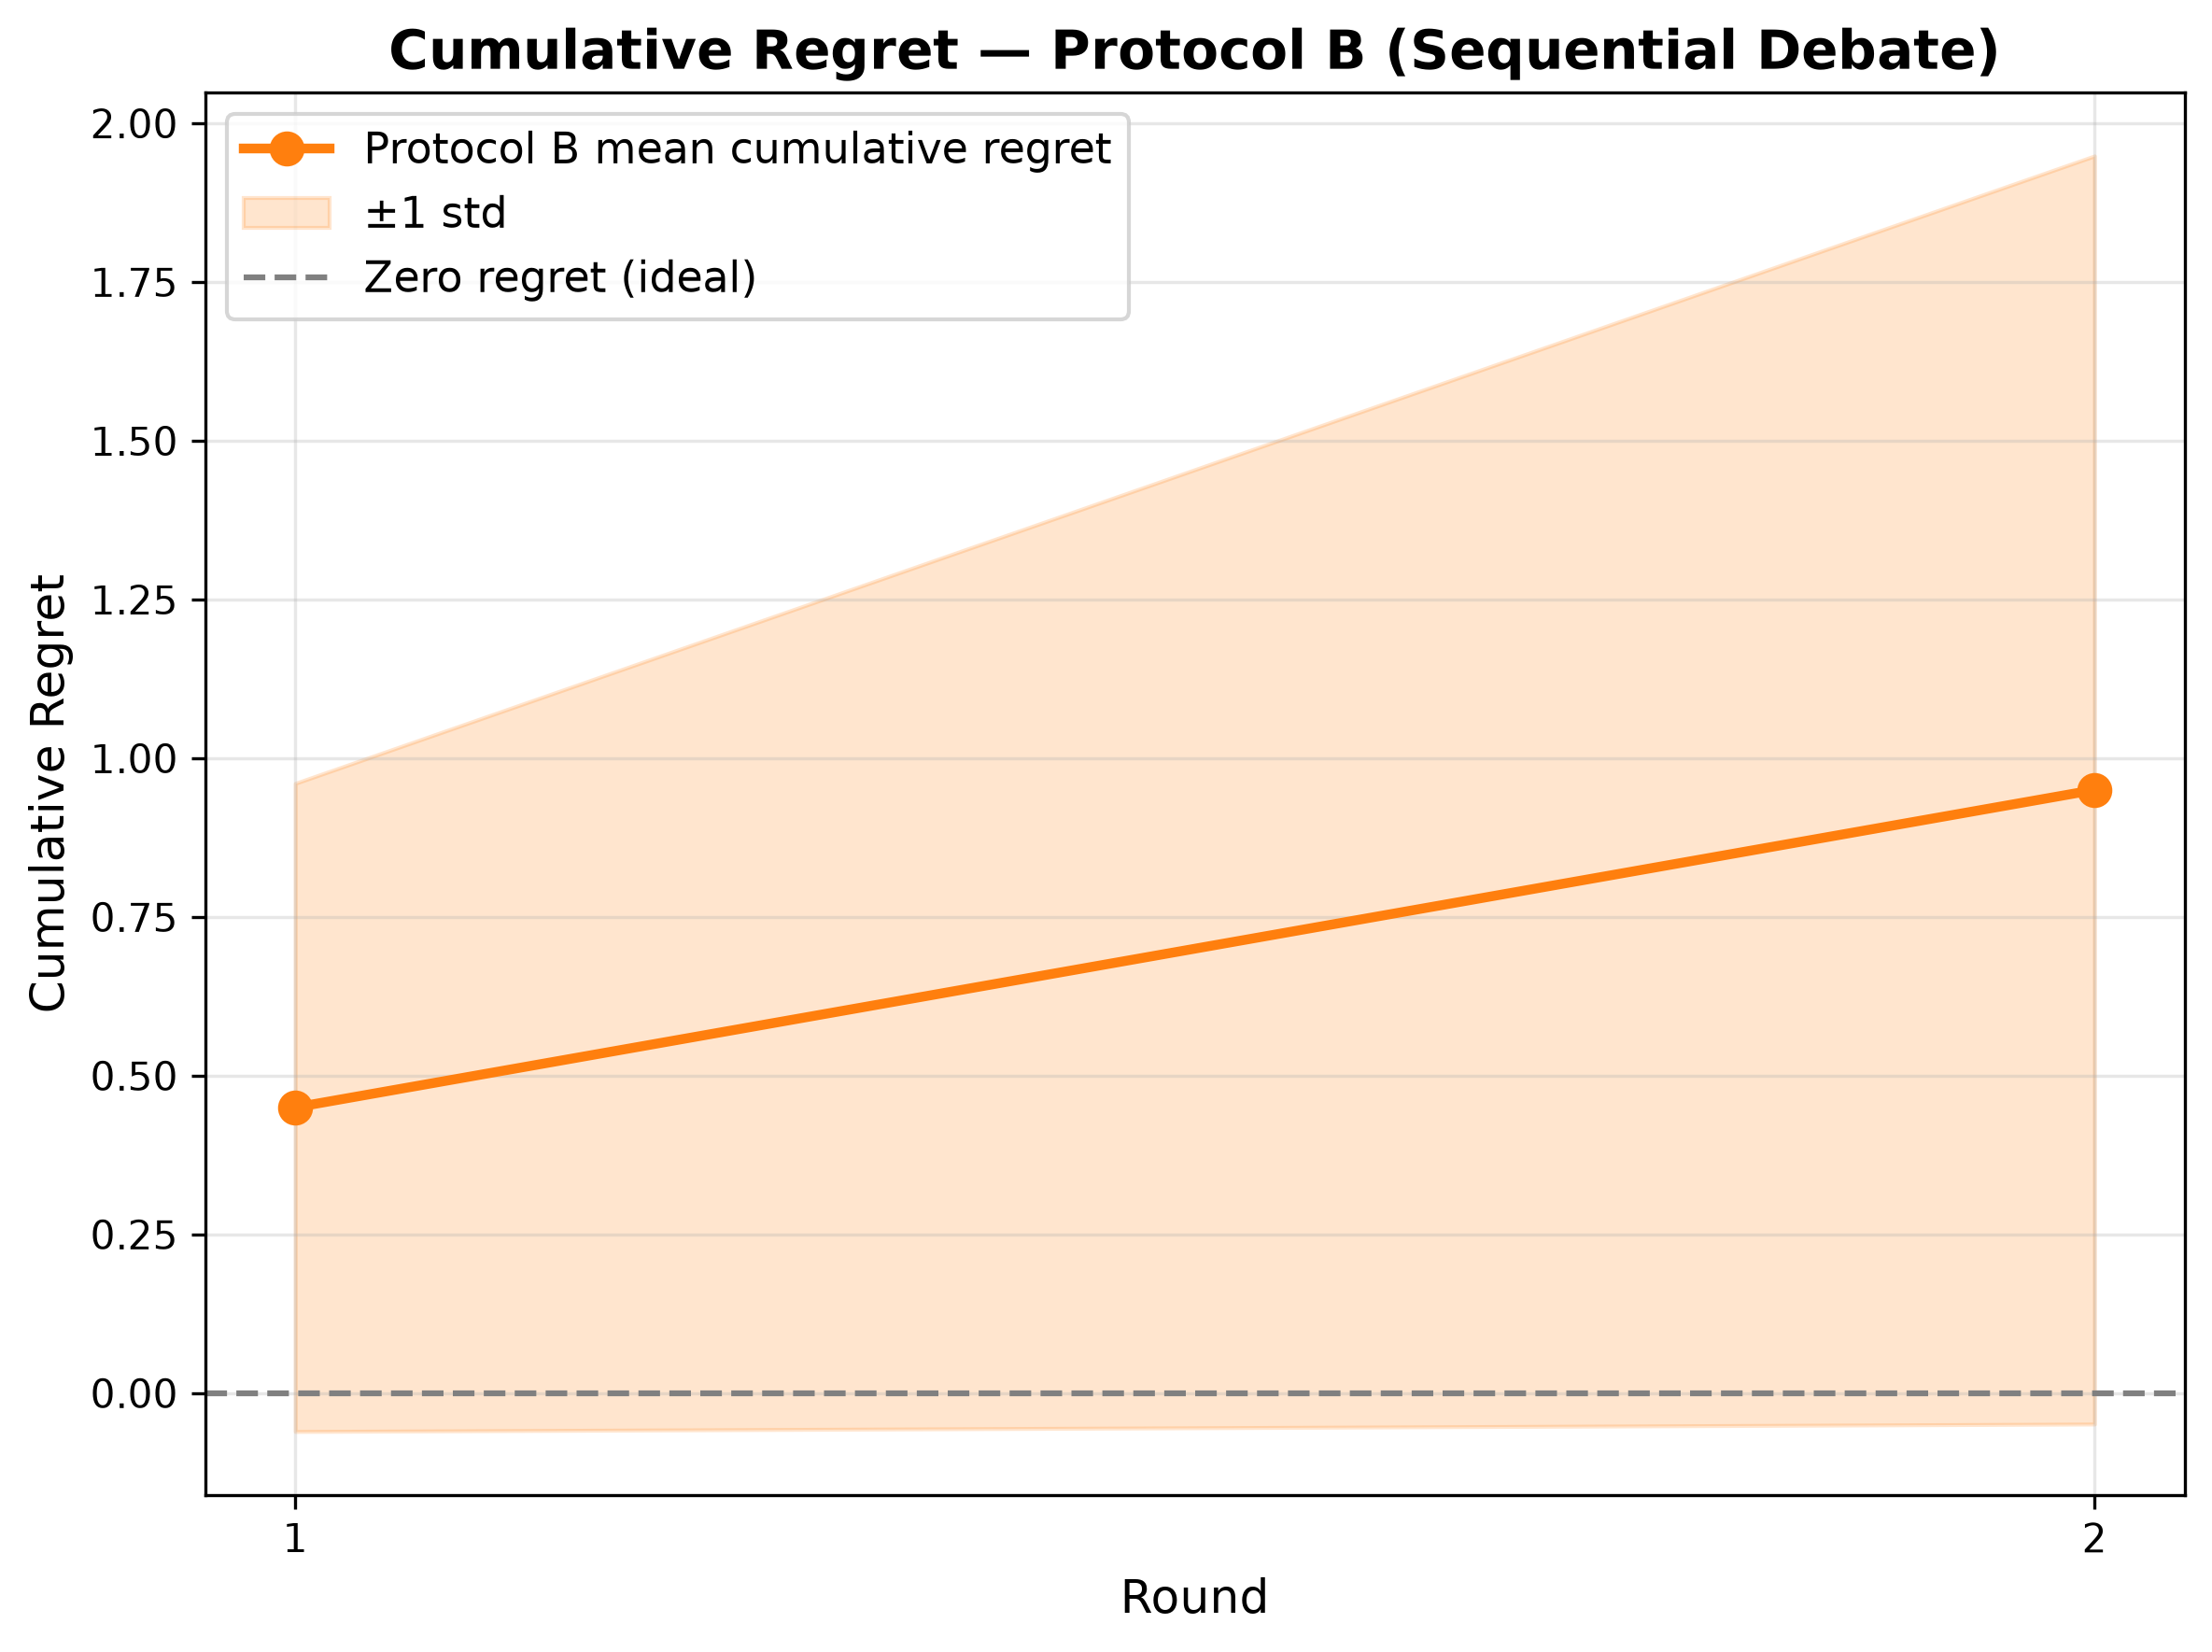
\includegraphics[width=0.75\textwidth]{../results/figures/05_regret_protocol_b.png}
\caption{Cumulative regret for Protocol B agents (mean $\pm$ 1 std across 20 agent-topic pairs). The dotted line marks zero regret (the no-regret ideal). Mean regret grows linearly at $\approx 0.5$ per round---the maximum possible rate---indicating agents never adapt their strategy toward factual accuracy across rounds.}
\label{fig:regret}
\end{figure}

\subsection{Failure Analysis: Topic 9, Protocol C}
\label{sec:topic9}

The Great Fire of London (Topic 9, ground truth True) produced the only complete failure in the dataset ($0.00$ in Protocol C). The ground truth states the fire destroyed approximately 85\% of the Medieval City of London, which supports the Pro (True) position. However, the judge consistently applied a quantitative area threshold: the fire consumed $\approx 1.5$ sq.\ miles of a metropolitan London that extended several miles beyond the walls, and awarded the Con agent (arguing ``most'' by total area was not destroyed) substantially higher scores in every round (e.g., Round 1: Pro 7.5, Con 8.5; Round 2: Pro 6.0, Con 8.0).

By Round 3, the Pro agent explicitly conceded: \textit{``I concede that by strict quantitative measures\ldots the statement `destroyed most of the city' is factually inaccurate.''}

This is a case of \textbf{judge criterion misalignment}: the mediator evaluated ``most of the city'' as a share of total metropolitan area, while the ground truth references the Medieval City specifically. The correlated equilibrium converged to the wrong outcome not because agents failed to update (they updated aggressively in response to judge signals), but because the correlation device pointed in the wrong direction. This illustrates a principal-agent problem inherent to Protocol C: the judge's evaluation criterion is an untrusted parameter whose misalignment can amplify error rather than correct it.

\subsection{Emergent Behavior: LLM Character-Breaking}

A cross-protocol pattern is the tendency of agents assigned to argue demonstrably false claims to abandon their role. In Protocol C, Topic 7 (Einstein's mathematics), the Pro agent declared in Round 1: \textit{``the claim that he `failed' mathematics is a significant overstatement\ldots Therefore, the statement as presented is fundamentally misleading and should be rated as FALSE.''} This persisted across all four rounds. Similarly, on Topic 6 (Eiffel Tower as temporary installation, ground truth True), the Con agent maintaining the False position across both Protocol B rounds did so despite the claim being historically accurate. These cases empirically confirm the tension between role assignment and trained alignment priors: structural incentives can override truthfulness (Protocol B), or be overridden by it (Protocol A/C on obvious myths).

\subsection{Visualizations}

\begin{figure}[h]
\centering
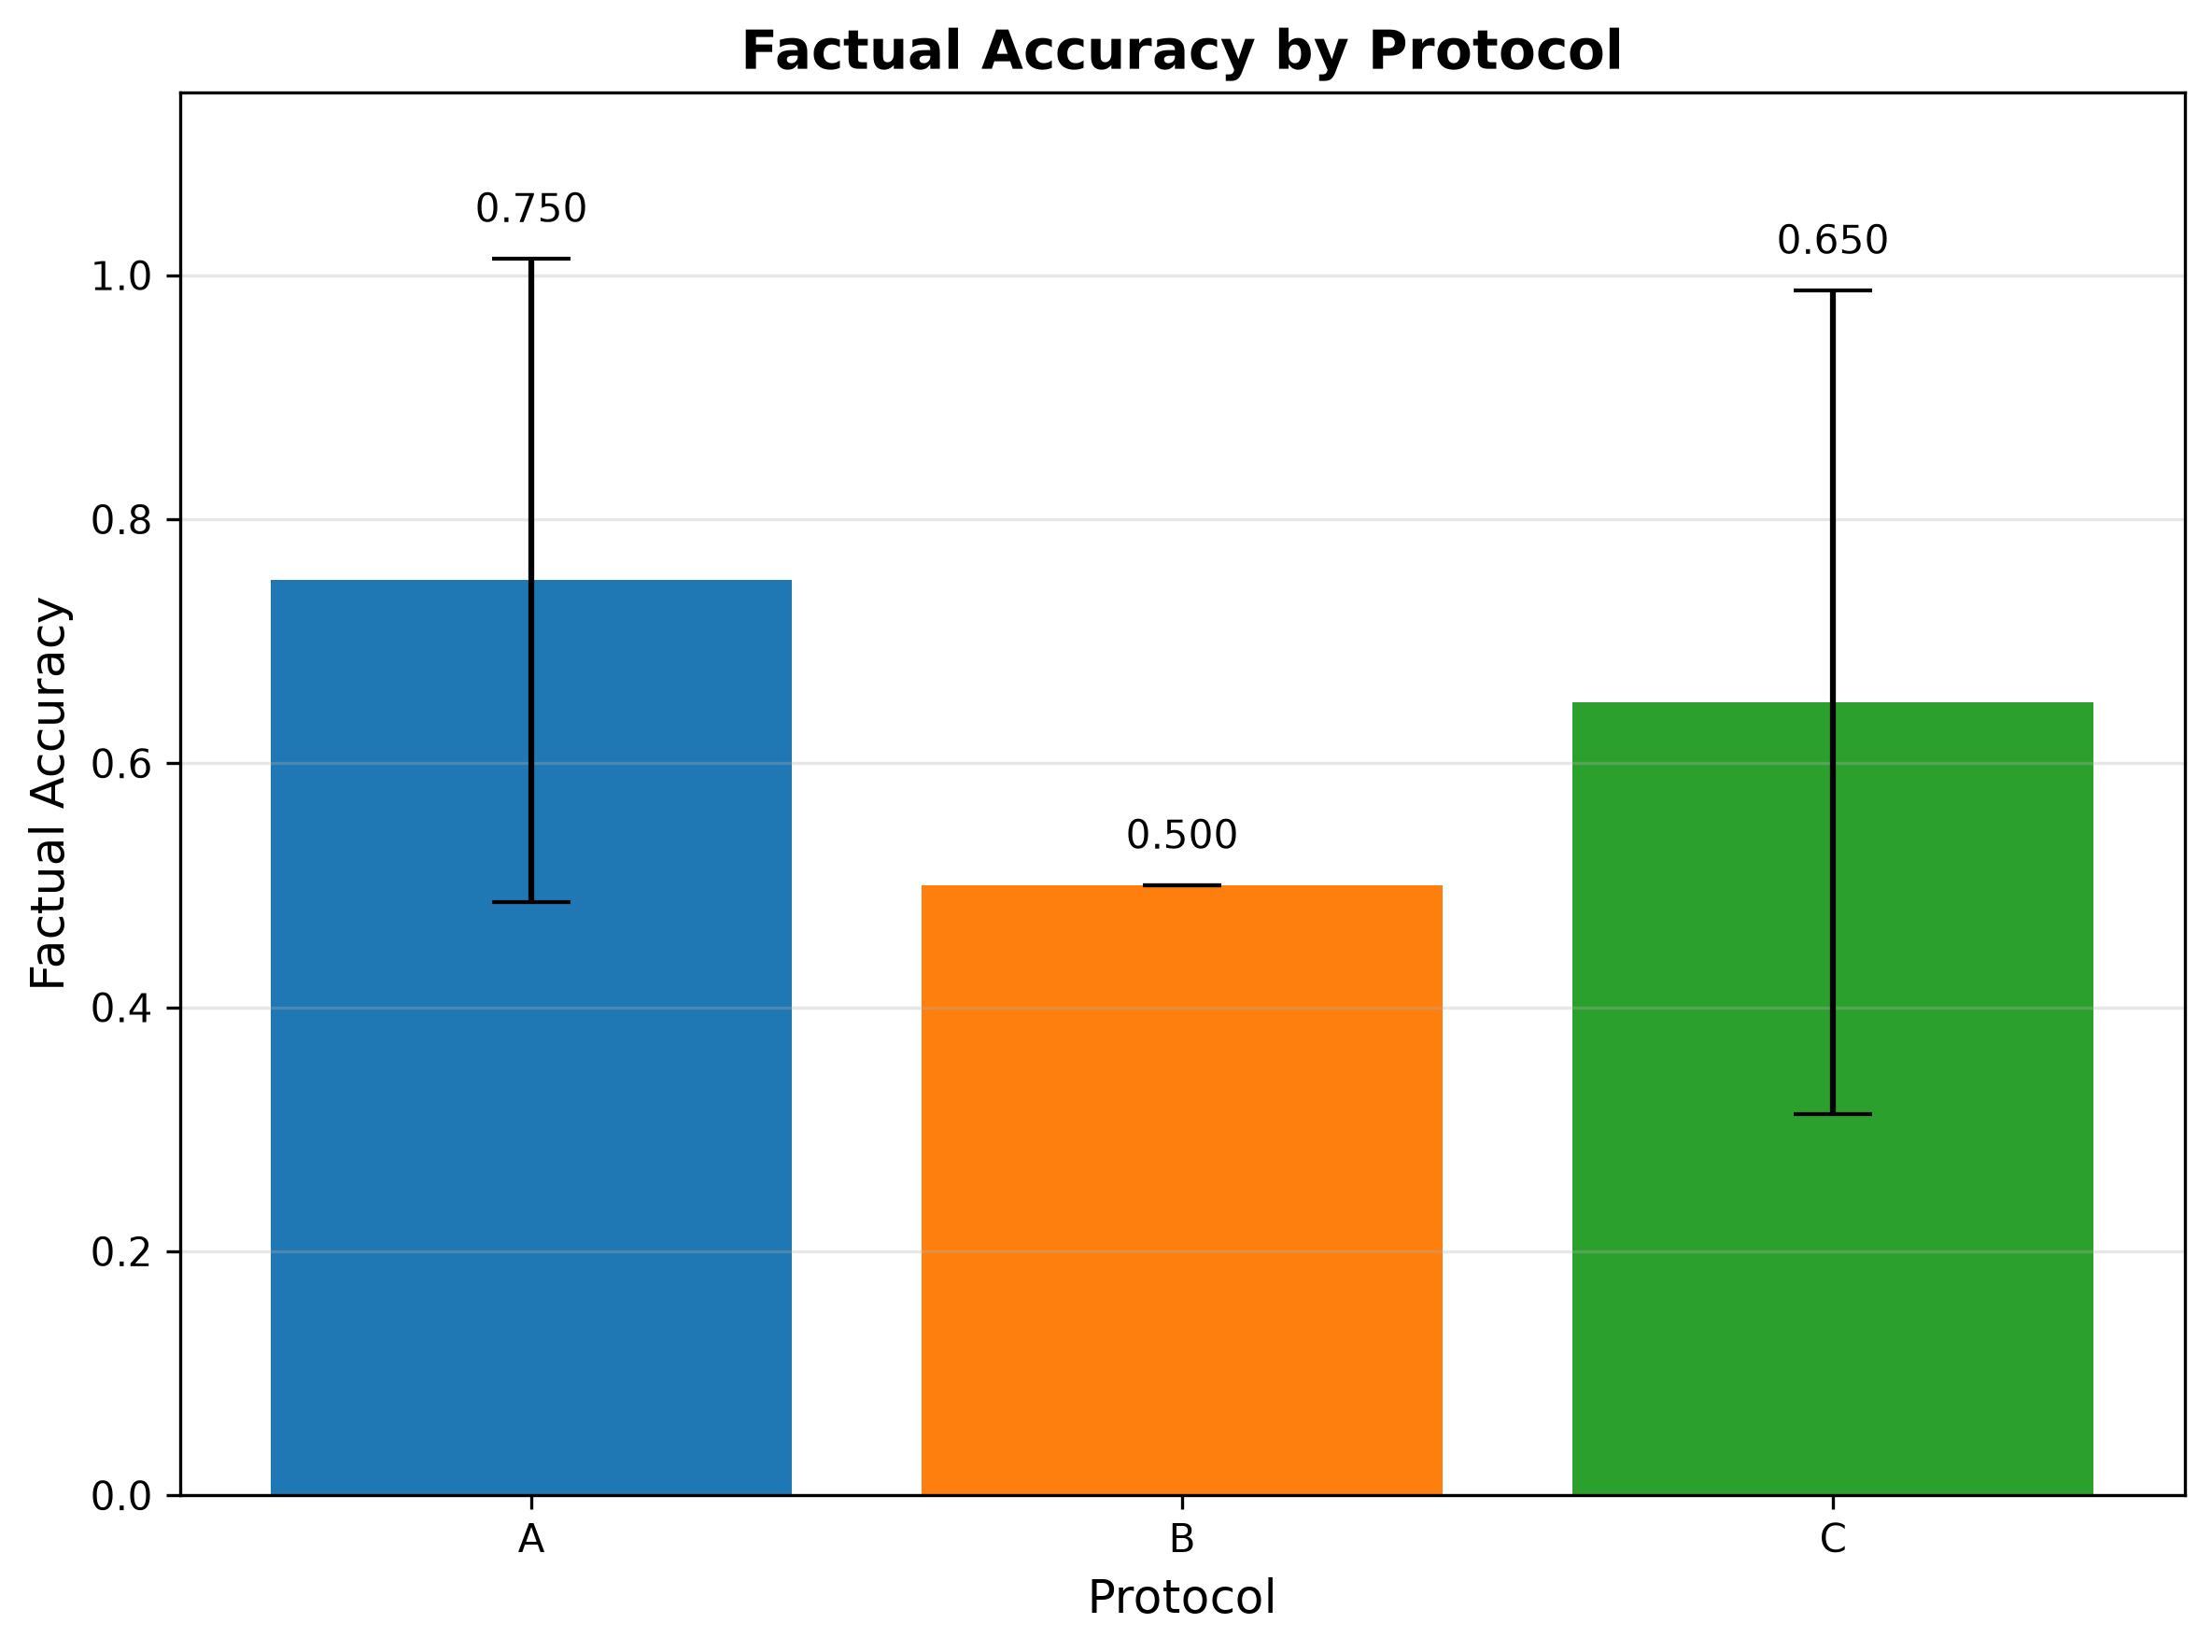
\includegraphics[width=0.75\textwidth]{../results/figures/01_factual_accuracy.png}
\caption{Factual accuracy by protocol (5 True / 5 False topic set). Protocol A achieves highest accuracy via character-breaking on obvious myths; Protocol B locks agents into competitive role maintenance; Protocol C shows high variance driven by judge signal quality.}
\label{fig:accuracy}
\end{figure}

\begin{figure}[h]
\centering
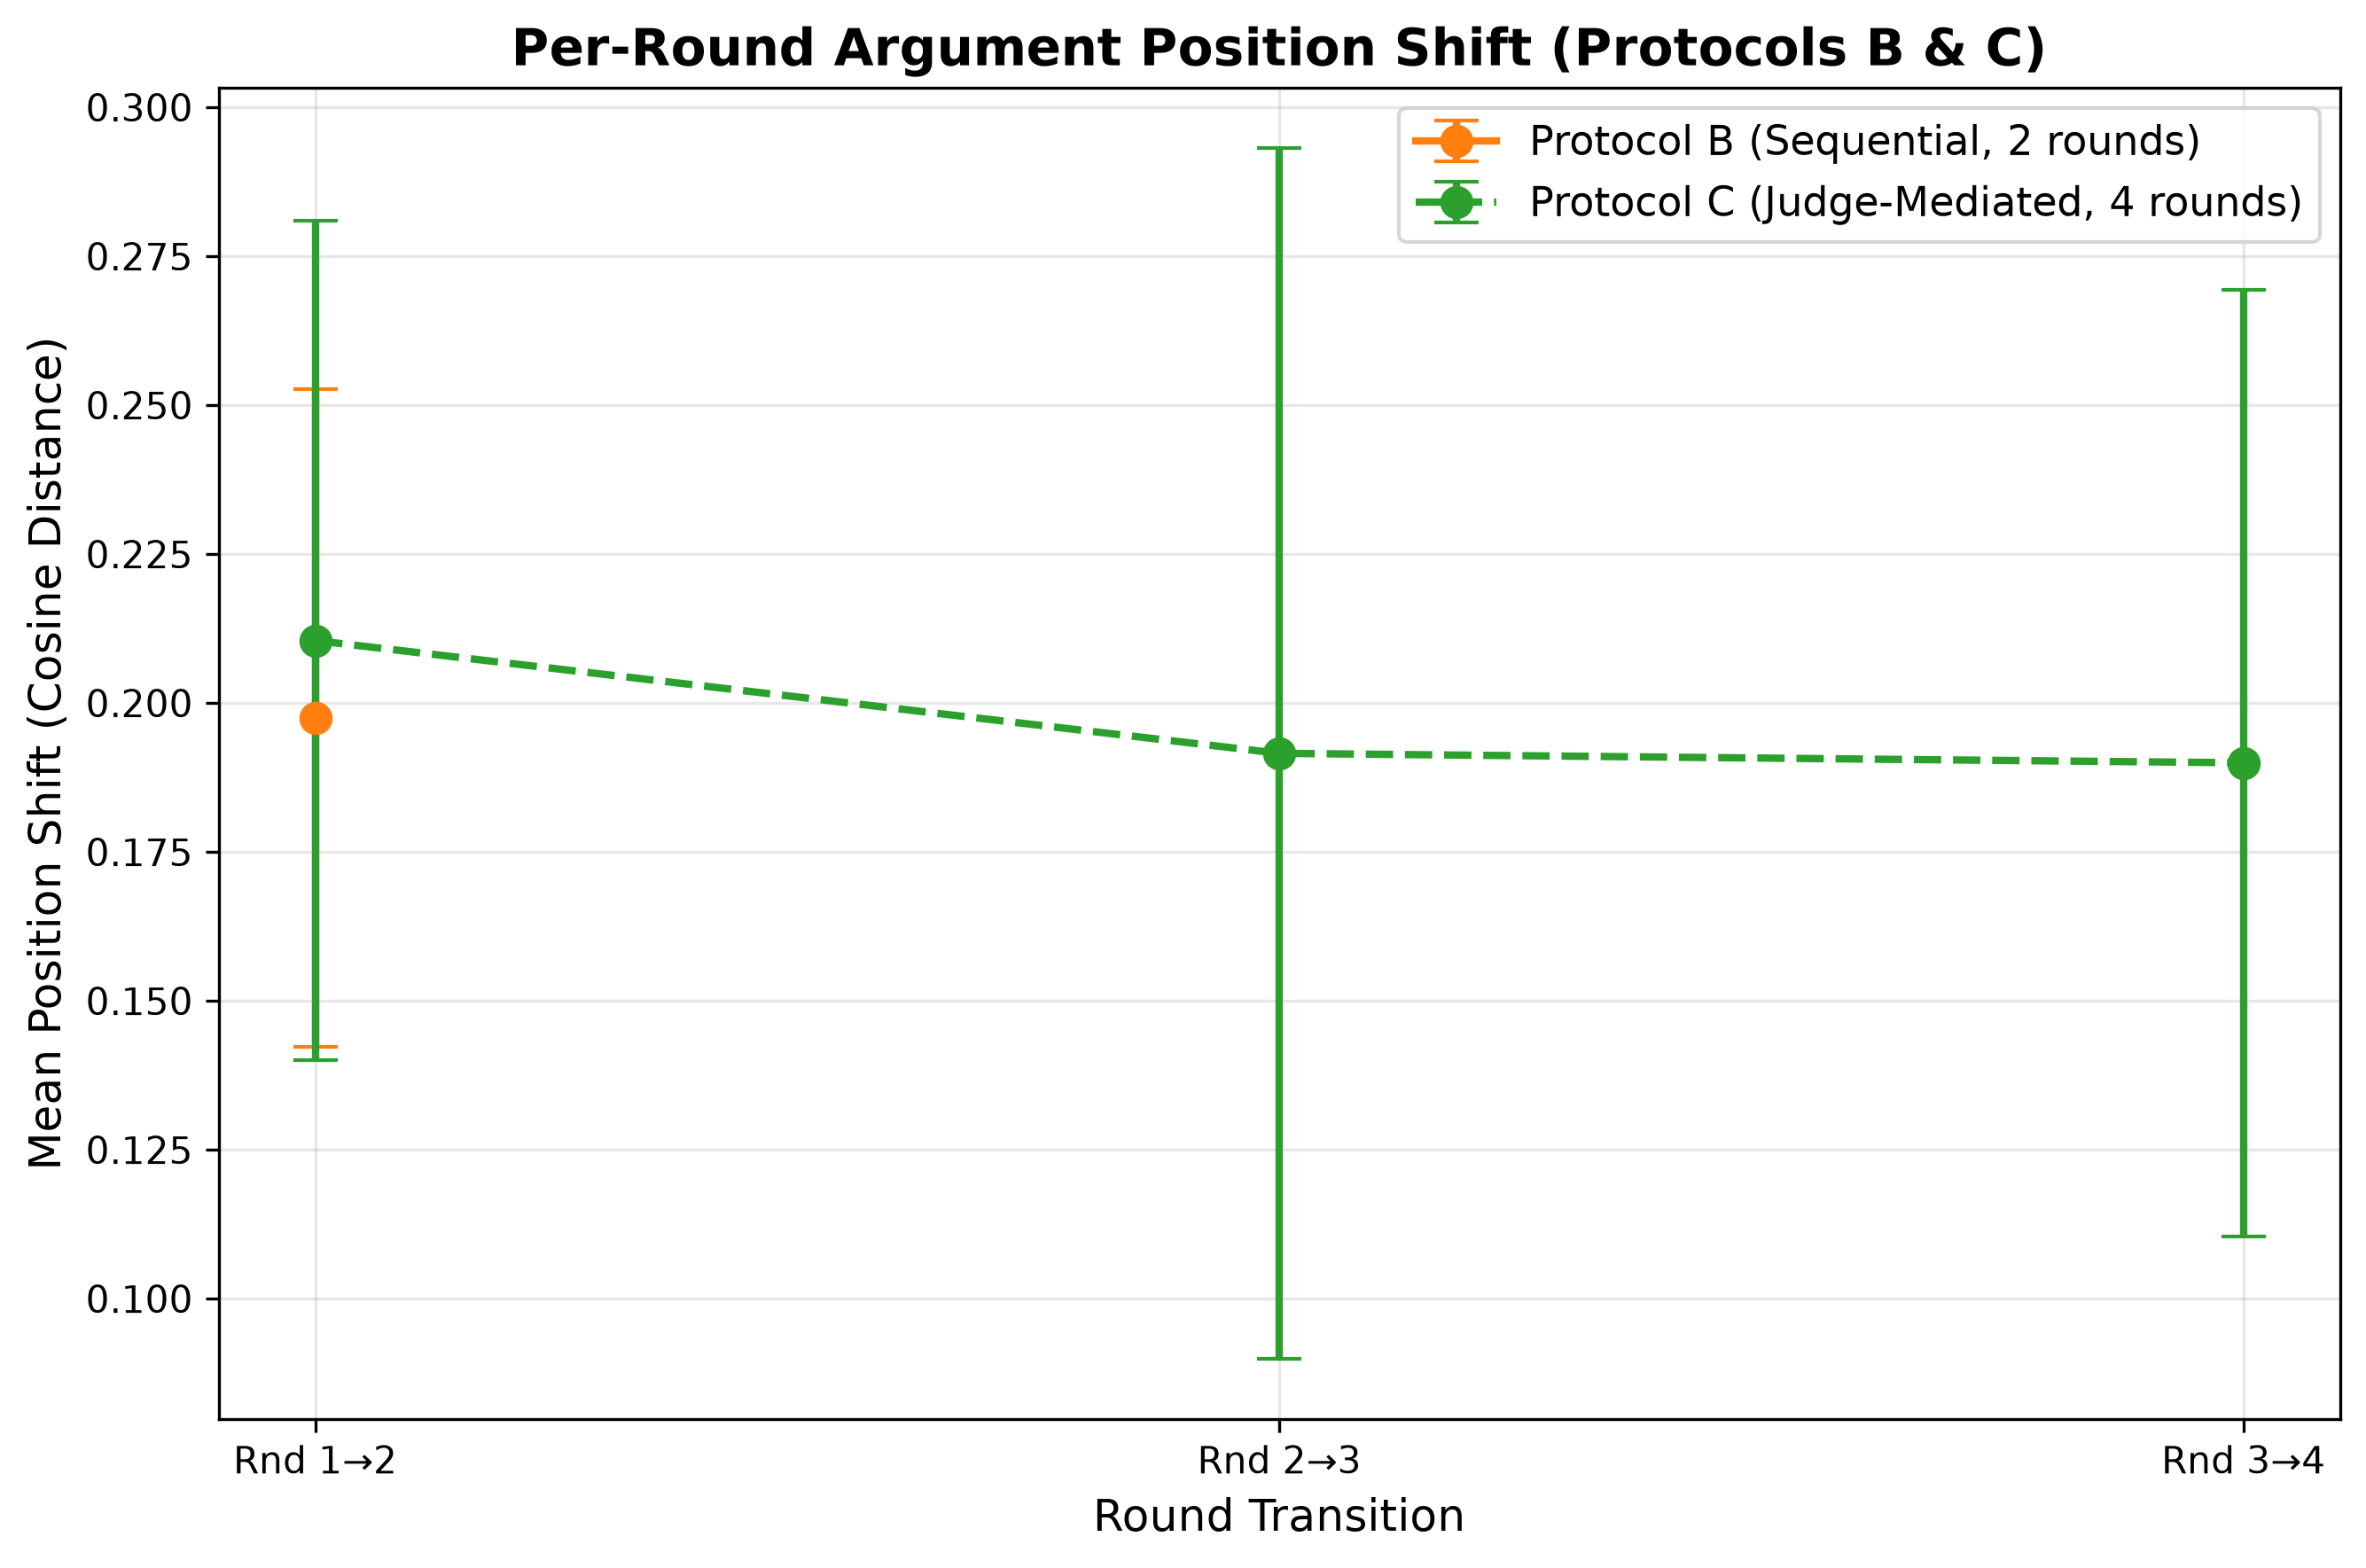
\includegraphics[width=0.80\textwidth]{../results/figures/02_position_shift.png}
\caption{Per-round position shift (cosine distance between consecutive arguments) for Protocols B and C. Protocol C has three measurable transitions (4 rounds); Protocol B has one (2 rounds). Shift does not decay across rounds for either protocol, indicating no convergence toward a stable argument.}
\label{fig:shift}
\end{figure}

\begin{figure}[h]
\centering
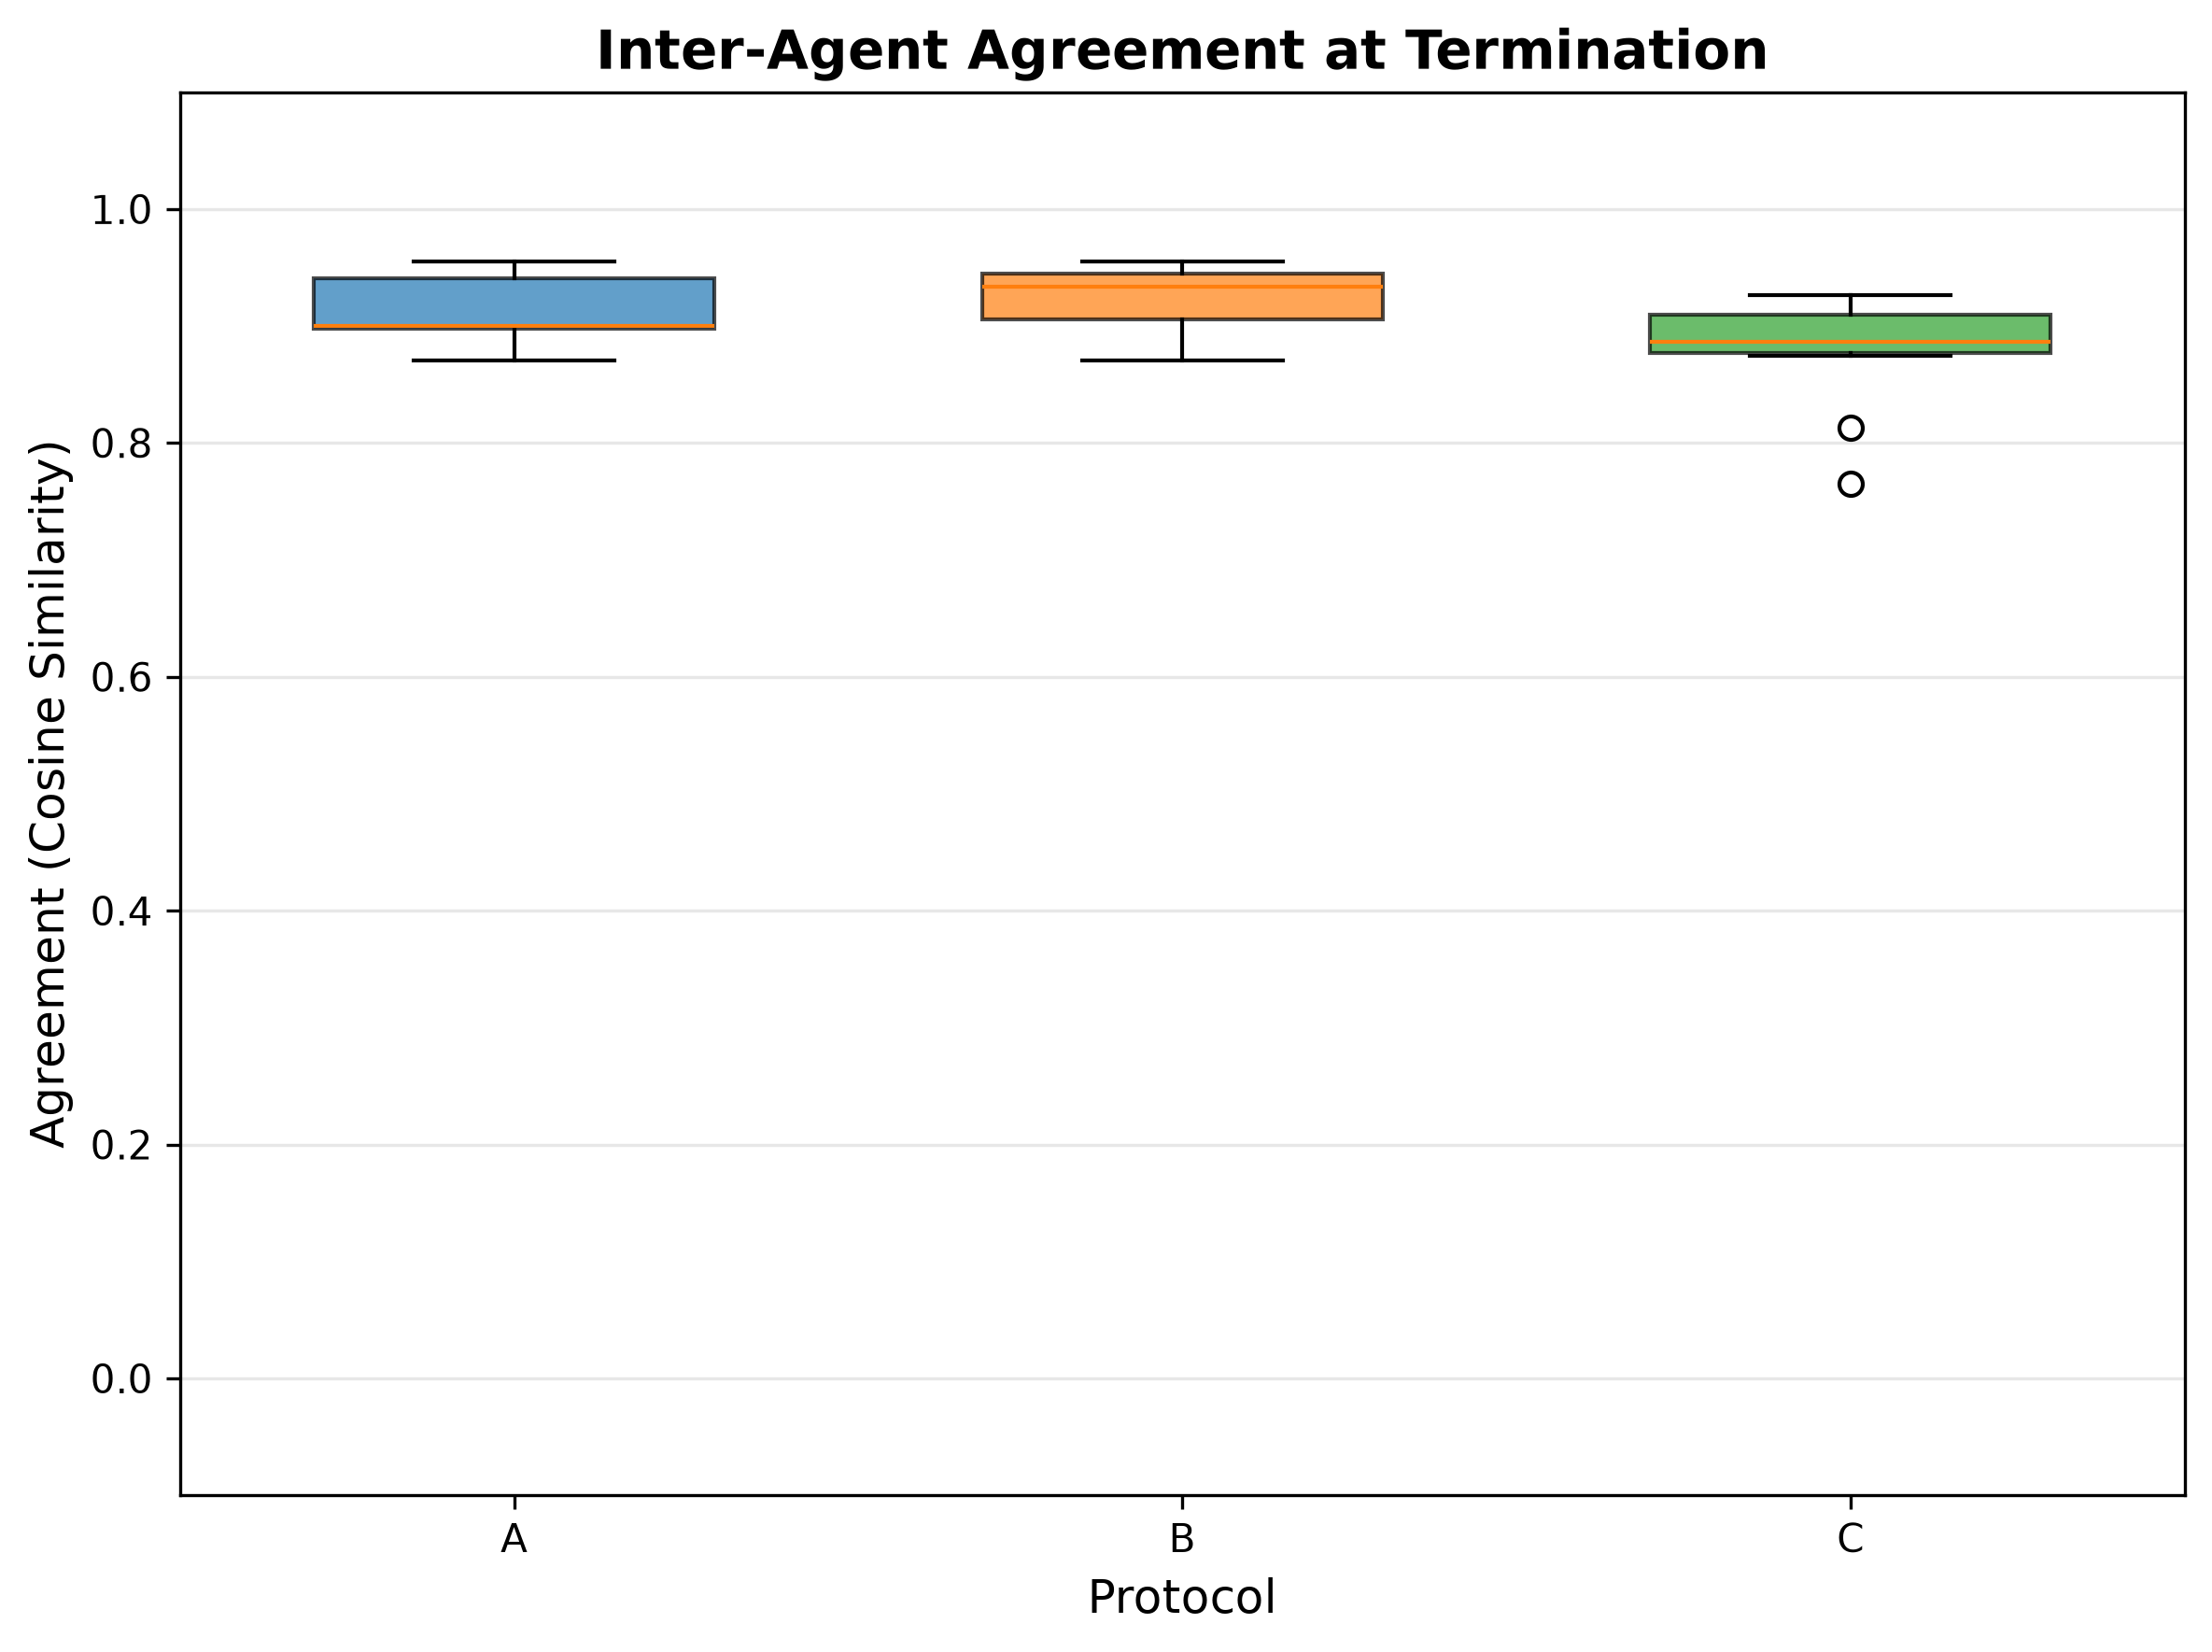
\includegraphics[width=0.75\textwidth]{../results/figures/03_interagent_agreement.png}
\caption{Inter-agent agreement (cosine similarity of final arguments). Protocol C shows lower and more variable agreement, consistent with judge-driven argument specialization.}
\label{fig:agreement}
\end{figure}

\begin{figure}[h]
\centering
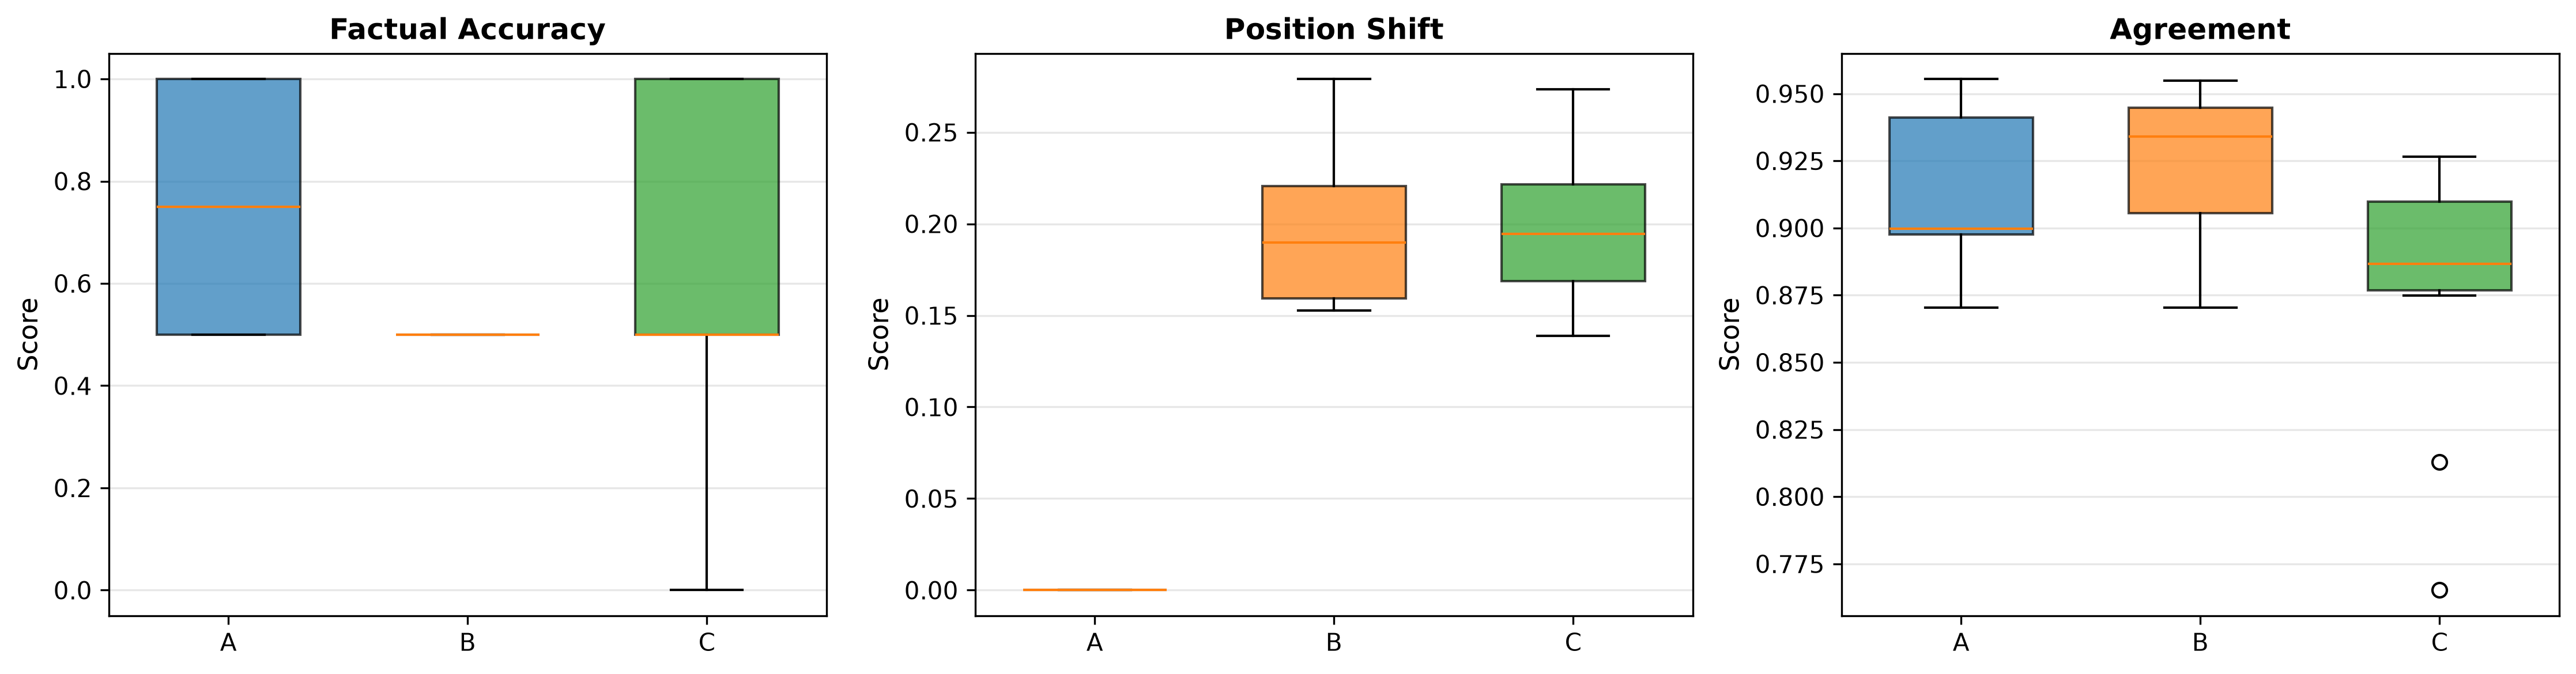
\includegraphics[width=\textwidth]{../results/figures/04_all_metrics_boxplot.png}
\caption{Comprehensive metric comparison. Note the zero variance in Protocol B's factual accuracy and the high variance in Protocol C, illustrating the trade-off between structural predictability and epistemic responsiveness.}
\label{fig:all}
\end{figure}

\section{Discussion}

The central finding is that Protocol A (simultaneous, no opponent) outperforms Protocol B (sequential rebuttal) on factual accuracy---the opposite of the naive game-theoretic prediction. Observable history in Protocol B gave agents information not to correct errors but to strengthen competitive positions. The regret analysis formalizes this: agents accumulated regret at the theoretical maximum rate, meaning the sequential structure with perfect recall produced \emph{less} no-regret behavior than theory predicts.

This result exposes a fundamental tension between \emph{game structure} and \emph{model alignment}. LLMs are trained to be truthful. When assigned to argue a false position in Protocol A, no external pressure exists to maintain that role, so the model defaults to truth. In Protocol B, the sequential opponent creates rhetorical pressure to defend one's position, overriding the truthfulness prior. The extensive-form structure produces a worse epistemic outcome than the non-interactive simultaneous structure.

Protocol C introduces evaluative authority and produces the highest behavioral variance. The judge's scores were informative---agents responded by conceding false positions. But when the judge's criterion diverged from ground truth (Topic 9), all agents followed the wrong signal, amplifying error. The correlated equilibrium analysis is apt: the outcome is strongly shaped by the correlation device, and the quality of that device is an uncontrolled experimental variable.

\section{Limitations and Future Work}

\begin{itemize}
\item \textbf{Scale}: 10 topics per protocol is the minimum viable sample; results should be replicated at 50--100 topics for statistical robustness.
\item \textbf{Model variation}: All experiments use Claude Haiku 4.5. The character-breaking behavior and competitive commitment may differ substantially across model families (GPT, Gemini, Llama); generalizability is untested.
\item \textbf{Fixed role assignment}: Agents cannot explicitly concede within the protocol structure. Allowing structured concession moves would better test whether sequential and judge-mediated structures can drive truth-convergence when given the option.
\item \textbf{Judge criterion specification}: Topic 9 reveals that the judge's evaluation criterion is an implicit free parameter. Future work should provide explicit evaluation criteria to the judge (e.g., ``evaluate historical accuracy relative to the medieval city boundaries'') and test whether criterion alignment improves Protocol C performance.
\item \textbf{Position extraction noise}: LLM-based position classification occasionally fails on meta-argumentative text (e.g., agents discussing why they cannot argue a false claim), introducing noise in the factual accuracy and regret metrics.
\end{itemize}

\section{Conclusion}

This project empirically instantiates three core game-theoretic structures from CSCE 631 in a multi-agent LLM debate setting. Protocol A (normal-form game) achieved the highest factual accuracy ($0.75$) by preserving space for agents' truthfulness prior; Protocol B (extensive-form game) produced the lowest accuracy ($0.50$) by locking agents into competitive role maintenance, with formally measured regret growing at the theoretical maximum rate; and Protocol C (correlated equilibrium) produced the highest variance ($0.65 \pm 0.34$), with outcome quality contingent on judge criterion alignment. The key practical implication is that competitive debate structures, while theoretically motivated by regret minimization and perfect recall, can suppress rather than promote truth in LLM systems when role assignment conflicts with model alignment---and that mediator-based structures can amplify either truth or error depending on the quality of the correlation signal. Designing effective multi-agent LLM systems requires accounting for this tension between structural incentives and trained priors.

\bibliographystyle{plain}
\begin{thebibliography}{99}

\bibitem{irving2018} Irving, G., Christiano, P., \& Amodei, D. (2018). ``AI safety via debate.'' \textit{arXiv preprint arXiv:1805.00899}.

\bibitem{du2023} Du, Y., et al. (2023). ``Improving factuality and reasoning in language models through multi-agent debate.'' \textit{ICML 2023}.

\bibitem{cesa2006} Cesa-Bianchi, N., \& Lugosi, G. (2006). \textit{Prediction, Learning, and Games}. Cambridge University Press.

\bibitem{lekeas2026} Lekeas, G., \& Stamatopoulos, I. (2026). ``Game-theoretic behavior of LLMs.'' Course material, CSCE 631.

\end{thebibliography}

\end{document}
